\documentclass[onlymath, nologo]{beamer}

\usepackage{amsmath, amsfonts}
\usepackage{tikz}
\usepackage{tabulary}
\usepackage{array}
{\renewcommand{\arraystretch}{2}%
\usepackage{mathtools}
\setbeamertemplate{caption}{\raggedright\insertcaption\par}
\usepackage{multimedia}
\usepackage[theorems, skins]{tcolorbox}

\graphicspath{{../figs/}}

\definecolor{UTBlue}{RGB}{94,156,174}
\definecolor{HCrimson}{RGB}{165,28,48}
\definecolor{HInk}{RGB}{30,30,30}
\definecolor{HMortar}{RGB}{140,129,121}
\definecolor{HParchment}{RGB}{243,243,241}
\definecolor{HSlate}{RGB}{137,150,160}
\definecolor{HShade}{RGB}{186,197,198}
\tcbset{colback=HParchment,colframe=HCrimson}

\usetheme[white]{Harvard}

\author[]{Instructor:  David Sondak \\ TFs:  Charles Liu, Eric Wu and Kevin Wu}
\title{CS207: Systems Development for Computational Science}
\subtitle{\url{https://iacs-cs-207.github.io/cs207-F17/}}

\institute{Harvard University \\ 
           Institute for Applied Computational Science}
\date{\large 8/30/2017}

\begin{document}

\bgroup
\makeatletter
\setbeamertemplate{footline}{}
\makeatother

  \begin{frame}
    \titlepage
  \end{frame}
  \egroup
  
  \setcounter{framenumber}{0}

  \begin{frame}{Motivation:  The Pillars of Science}
    \includegraphics<1>[width=\textwidth]{old_pillars.pdf}
    \includegraphics<2>[width=\textwidth]{new_pillars.pdf}
  \end{frame}

  \begin{frame}{Computational Science}
    \vspace{-0.8em}
    \begin{center}
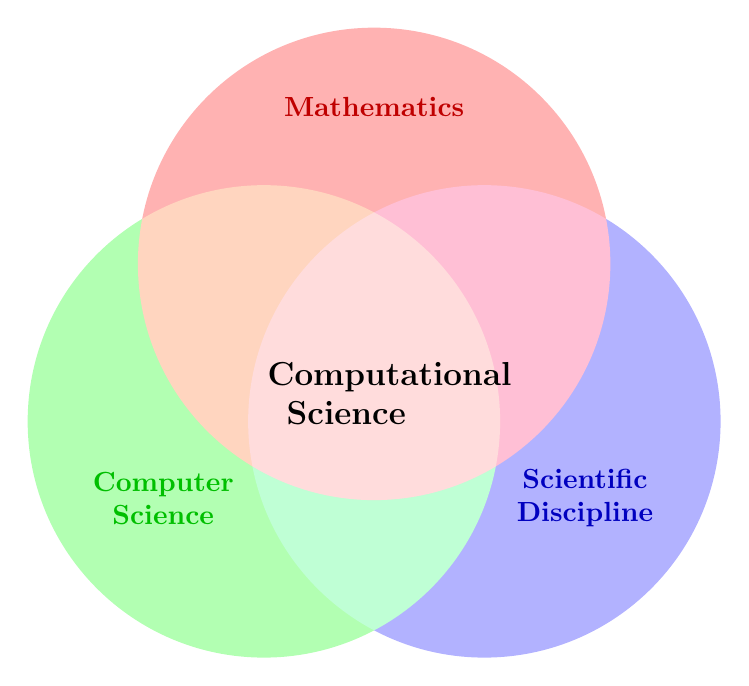
\begin{tikzpicture}
  \begin{scope}[blend group = soft light]
    %\fill[red!30!white]   ( 90:2.0) circle (3);
    %\fill[green!30!white] (160:2.0) circle (3);
    %\fill[blue!30!white]  (20:2.0) circle (3);
    \fill[red!30!white]   ( 90:2.0) circle (3);
    \fill[green!30!white] (180:1.4) circle (3);
    \fill[blue!30!white]  (360:1.4) circle (3);
  \end{scope}
  \node at ( 90:4)    {\textcolor{red!75!black}{\textbf{Mathematics}}};
  \node [text centered, text width = 2cm] at (200:2.85)   {\textcolor{green!75!black}{\textbf{Computer Science}}};
  \node [text centered, text width = 2cm] at (340:2.85)   {\textcolor{blue!75!black}{\textbf{Scientific Discipline}}};
  \node [font=\large, text centered, text width = 2cm] at (135:0.5) {\textbf{Computational Science}};
\end{tikzpicture}
\end{center}

  \end{frame}

  \begin{frame}{Why take this class?}
    \begin{columns}[T]
      \begin{column}{0.7\textwidth}
        \begin{itemize}
          \item Scientific software is complex 
          \item Your code needs to be:
            \begin{itemize}
              \item Reuseable 
              \item Portable 
              \item Robust
            \end{itemize}
          \item Must go beyond ``scripting'' \\[1.0em]
        \end{itemize}
        \vfill
        \uncover<3->{
        \begin{tcolorbox}[title=CS207 Objectives, arc is angular]
            \centering
            To give students who may not have a 
            traditional computer science background the knowledge 
            and tools to develop and maintain effective software 
            for computational science applications.
        \end{tcolorbox}
        }
      \end{column}
      \begin{column}{0.3\textwidth}
        \includegraphics<2->[width=\textwidth]{frustrated_coder.jpg} \hfill \\[1.0em]
        \includegraphics<4->[width=\textwidth]{happy_coder.jpg}
      \end{column}
    \end{columns}
  \end{frame}

  \begin{frame}{Who should take this class?}
    \begin{itemize}
      \item Any kind of scientist is welcome to take this class! \\[1.0em]
      \item This course is computer science for people who aren't computer scientists:
      \begin{itemize}
        \item Data scientists
        \item Biologists
        \item Chemists
        \item Engineers 
        \item Physicists
        \item Mathematicians
        \item Economists
        \item \hspace{2.0em} \vdots %\\[1.0em]
      \end{itemize}
      \item It is also for computer scientists who want to develop scientific software \\[1.0em]
      \item CS207 is for students who need to know effective and modern software practices for 
            their career
    \end{itemize}
  \end{frame}

  \begin{frame}{Sample Topics}
    \uncover<1->{
      A few selected topics to be covered:
      \begin{columns}[T]
        \begin{column}{0.5\textwidth}
          \begin{itemize}
            \item Version control
            \item Python (basics)
            \item How Python works
            \item Software documentation
          \end{itemize}
        \end{column}
        \begin{column}{0.5\textwidth}
          \begin{itemize}
            \item Software testing
            \item Object-oriented programming
            \item Data structures
            \item Databases
          \end{itemize}
        \end{column}
      \end{columns}
      \vfill
    }
    \uncover<2->{
      \begin{columns}[b]
        \begin{column}{0.5\textwidth}
          Other potential topics \\ (not guaranteed):
          \begin{itemize}
            \item Debuggers and debugging
            \item Build systems (Make files, autotools, ...)
            \item Compiled languages
            \item Navigating a Unix OS
          \end{itemize}
        \end{column}
        \begin{column}{0.5\textwidth}
          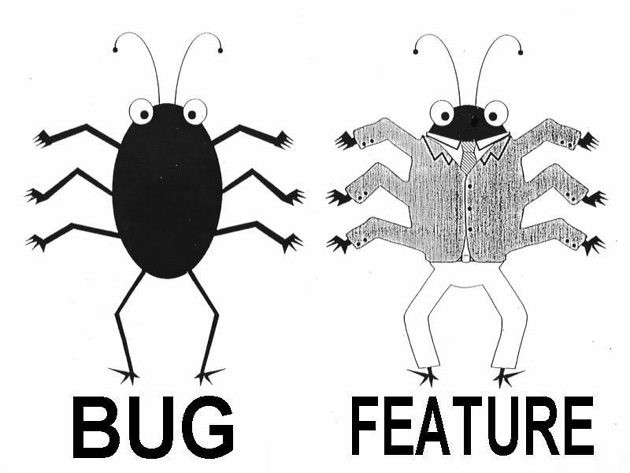
\includegraphics[width=\textwidth]{bug.jpg}
        \end{column}
      \end{columns}
    }
  \end{frame}

  \begin{frame}{Course Structure}
    \begin{itemize}
      \item CS207 is an application-driven course \\[0.5em]
      \item Two, $1.5$ hour lectures per week \\[0.5em]
      \item Lectures centered around group programming exercises using Jupyter notebooks  \\[0.5em]
      \item ``Weekly'' programming assignments for homework \\[0.5em]
      \item Primary deliverable is a software development project \\[0.5em]
      \item All course content hosted on GitHub
    \end{itemize}
    \vfill
    \centering
    \Large Course Website:  \url{https://iacs-cs-207.github.io/cs207-F17/}
  \end{frame}

  \begin{frame}{Course Project:  Overview}
    \begin{itemize}
      \item You will work in groups of $3$ to $4$ people (assigned by teaching staff) \\[0.75em]
      \item You will add to your library throughout the semester \\[0.75em]
      \item You will demo your progress for a midterm presentation  \\[0.25em]
        \begin{itemize}
          \item Includes a proposal of your final project \\[0.75em]
        \end{itemize}
      \item For the final project, you will add a non-trivial feature to your library \\[0.75em]
      \item A portion of your grade will come from peer-assessment \\[0.75em]
      \item Exact details on website
    \end{itemize}
  \end{frame}

  \begin{frame}{Course Project:  The Topic}
    \begin{itemize}
      \item We will write a chemical kinetics library!
    \end{itemize}
    \begin{columns}[c]
      \begin{column}{0.5\textwidth}
        \centering
        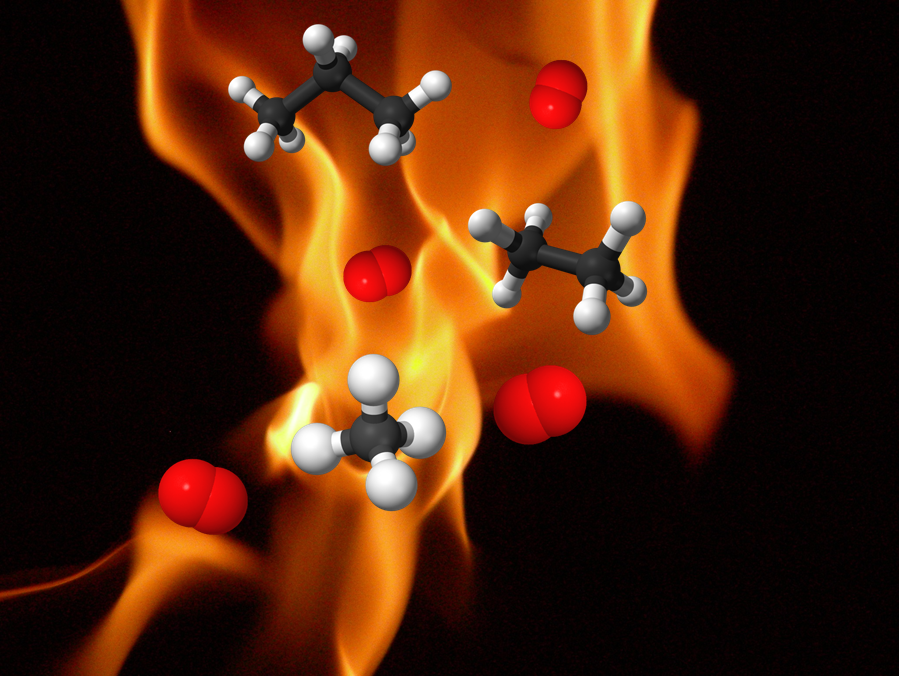
\includegraphics[width=\textwidth]{combustion.png} \hfill \\
        \tiny Combustion Kinetics Course, Technische Universitat Berlin
      \end{column}
      \begin{column}{0.5\textwidth}
        \centering
        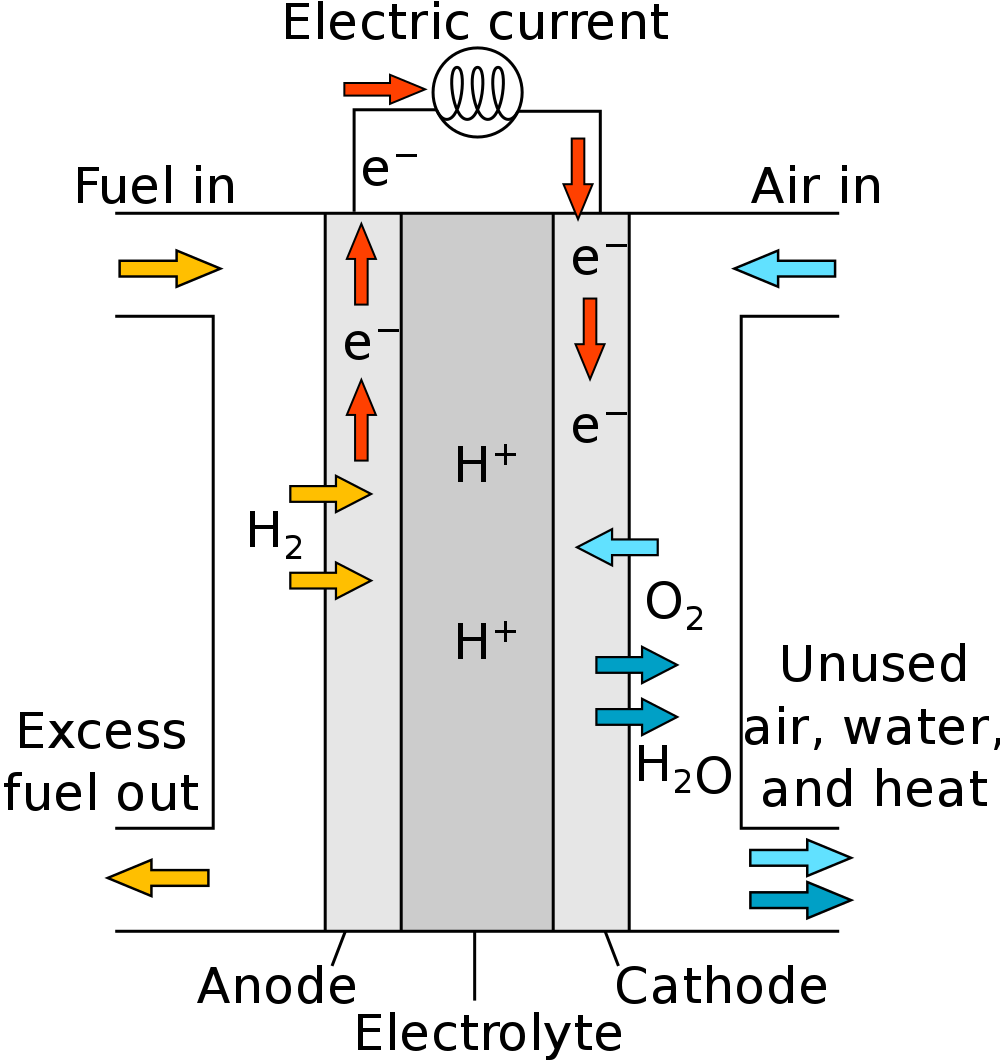
\includegraphics[width=\textwidth]{PEM_fuel_cell.png} \hfill \\
        \tiny \url{https://commons.wikimedia.org/wiki/File:Proton_Exchange_Fuel_Cell_Diagram.svg}
      \end{column}
    \end{columns}
  \end{frame}

  \begin{frame}{Course Project:  Why Kinetics???}
    \begin{itemize}
      \item The mathematics is accessible
      \begin{align*}
        \frac{\mathrm{d}\mathbf{x}}{\mathrm{d}t} = 
          \underbrace{\textcolor{HCrimson}{\mathbf{f}\left(\mathbf{x}, T\right)}}_{\textrm{return this}}
      \end{align*}
      \item Very popular area of study \\[0.25em]
        \begin{itemize}
          \item Examples in physics, engineering, machine learning, and data science \\[1.0em]
        \end{itemize}
      \item Good, clean, non-trivial example for illustration of software development principles \\[1.0em]
    \end{itemize}
    \begin{tcolorbox}[title=Important Note on Expectations, arc is angular]
        \centering
        You are not responsible for becoming an expert in chemical kinetics!  You will not be tested 
        on your kinetics proficiency.
    \end{tcolorbox}
  \end{frame}

\end{document}
